\chapter{Is it All Good in the Neighborhood? How Partisanship May Shape Evaluations of Municipal Services}
\label{chap:chapter2}

While extensive work has been done examining how voters evaluate the performance of federal and state governments, comparably less attention has been paid to evaluations in the context of local governments. In what work has been done, researchers often focused on small geographical areas and how information availability shaped evaluations \citep[e.g.,][]{berryAccountabilityLocalElections2007,paysonWhenAreLocal2017}. We still know relatively little about how voters' individual-level characteristics shape how they evaluate their local governments and their respective services. Nor do we know whether these evaluations correlate to the actual performance of local governments. Traditional conceptions of local politics might suggest that these evaluations are primarily a result of voters' day-to-day interactions with these services \citep[e.g.,][]{kaufmannUrbanVoterGroup2004,yoderDoesPropertyOwnership2020}; however, this framework fails to take into account the growing role partisan identities play in voter's evaluations of government services at state and federal levels \citep{healyRetrospectiveVotingReconsidered2013}. Furthermore, the increasing nationalization of politics means local political issues are no longer as insulated from traditional partisan discourse as previously conceived \citep{hopkinsIncreasinglyUnitedStates2018}.

In this article, I attempt to further our understanding of how voters evaluate their local government's performance and the role partisan identities play in constructing these evaluations. I argue that local services can become polarized when local issues become nationalized and distinct partisan cleavages form in the national discourse. For these polarized services, partisanship becomes a powerful identity through which individuals construct their local evaluations. This partisan lens then biases assessments of these services toward their party's average position regarding the service.

To test this argument, I use a nationally representative and geographically diverse survey that asks individuals to grade two prominent local services, schools, and police. While both are primarily under the purview of local governments and receive significant political attention, they differ regarding their partisan division. Using administrative records from the Census Bureau and National Weather Service, I then match all respondents to their local governments. This matching allows me to, in addition to gathering respondent-level characteristics,  (1) account for locality-based effects that may influence a respondent's evaluation and (2) assign each respondent an objective measure of both services to isolate any form of partisan bias. 

Overall, I find a significant partisan bias in voters' evaluations of polarized services even after accounting for objective performance and prominent socio-economic features. Despite living in areas with similarly performing police agencies, Republicans systematically rate local police higher than Democrats and Independents. Notably, this bias is equivalent to a substantial change in objective outcome measures for police and the effects of income and race. While I find differences in how partisans evaluate local schools, the results are comparably small and outweighed by school performance. To test the robustness of my results, I subset my data set to only large cities to incorporate additional city-specific measures, alternative local services, and city and state levels of partisan control. I find support for my theory, and interestingly, my results suggest that the partisan bias is based on national partisan preferences rather than on party control of the government.

This research contributes to the growing literature on the role of partisanship within local politics and provides further evidence of the nationalization of American politics. Notably, my research is one of relatively few to map a geographically diverse collection of specifically local evaluations to their respective municipalities. My results highlight how local services, like national policy issues, can become polarized and susceptible to partisan biases. These partisan effects are especially problematic as they can influence an individual's evaluations more than a local service's objective performance. Additionally, these results have potential implications for the already low levels of accountability found with local politics, as voters may rely more on national opinion rather than local conditions when constructing their evaluations.



\section{The Process of Polarization}
I argue that some local services have become polarized due to the nationalization of American politics \citep{hopkinsIncreasinglyUnitedStates2018} and the adoption of services as party-owned issues. Borrowing from both the polarization \citep[e.g.,][]{levenduskyPartisanSortHow2010,sinclair2006party} and issue ownership literatures \citep[e.g.,][]{petrocikIssueOwnershipPresidential1996,egan2013partisan,green2004partisan}, I define a local service as polarized when parties hold ideologically distanced and distinctly homogeneous opinions regarding a service's intended purpose, appropriate support, and overall performance. Services can become polarized as the ideological distances of elite and media rhetoric surrounding a service increase \citep{prior2013,fiorinaPoliticalPolarizationAmerican2008,wilsonPolarizationContemporaryPolitical2020}. As more apparent partisan stances towards a service emerge, individuals' opinions of a service slowly converge to that of their party \citep{walgraveIssueOwnershipStability2009,walgravedimissue2012,craigWhoOwnsWhat2020}. A local service can become effectively polarized when this sorting becomes severe enough (i.e., there is little to no overlap in party positions). After polarization, individuals have apparent partisan affiliations and party positions to lean on when constructing their evaluations.

However, we know from past and recent research that not all aspects of local politics hold national significance or are inherently political \citep{anziaPartyIdeologyAmerican2021}. While some services and issues may intersect with national policy matters, such as education, law enforcement, and criminal justice, others remain distinctly local, like road management and zoning \citep{thompsonHowPartisanLocal2020,jensenCityLimitsPartisan2021,sancesWhenVotersMatter2021}. As a result, we should not anticipate uniform polarization in local services. Instead, the process should occur on a service-by-service basis.

Furthermore, we understand that the extent to which any aspect of politics aligns with an individual's political identity depends on the salience of its respective issues areas \citep{belangerIssueSalienceIssue2008a}. Local political outcomes, in particular, often require a catalyst for individuals to establish political connections and pay attention \citep{mooreMotivationsMobilizationComparing2022,nuamahCloseHomePlaceBased2021}. Previous research on local accountability suggests that news coverage or a political spotlight on a particular service is necessary for individuals to make political associations with that service \citep{paysonWhenAreLocal2017,berryAccountabilityLocalElections2007,debenedictis-kessnerStrategicGovernmentCommunication2022}. Therefore, services with broad relevance to many individuals and receiving sufficient media and political attention should be the most likely to become polarized. 

\subsection{How Partisanship Shapes Evaluations}
A fundamental assumption of my argument is that polarization and party identity shape individuals' evaluations of government performance. We know individuals craft their political opinions through their party identification \citep{campbellAmericanVoter1980,zallerjohnNatureOriginsMass1992} and that given the increasing alignment of ideological and policy preferences, an individual's overall evaluation tends to correspond to either that of their party's elites or their party's average position \citep{lenzLearningOpinionChange2009,sinclair2006party}. Past research in retrospective voting provides greater insight into why this is and its mechanisms. First, when individuals interpret policy outcomes, they must decide how to allocate blame or credit. Voters tend to attribute positive outcomes to their own party's performance and blame adverse outcomes on the other party \citep{healyRetrospectiveVotingReconsidered2013}. In the context of a local service, such as police, which may not belong to a specific party, Republican individuals may associate them more with their party. Thus, any negative performance on their behalf may be attributed to other political actors.

Second, partisanship can be used as a powerful heuristic when it is unclear how to interpret policy outcomes or establish lines of responsibility. In a study examining retrospective voting in the wake of Hurricane Katrina, \citet{malhotraAttributingBlamePublic2008} find that individuals were more likely to blame Republican officials for the deaths and damages resulting from the storm. However, these effects disappeared when respondents received the Republican official's title. There is also evidence that when information environments become polarized, individuals are more likely to adopt partisan cues even in the presence of contradictory objective information \citep{druckmanHowElitePartisan2013}. Thus, when tasked with evaluating police performance, individuals may rely more heavily on their partisan identity than objective performance. 


\subsection{Why Schools and Police}
Ideally, to analyze how local services become polarized, I could use longitudinal data on individual evaluations of various local services. Then, as services become polarized in the national sphere, I could measure the divergence between partisans. Unfortunately, no such data is sufficiently detailed to ask about local services or cover an extended time frame. An alternative way to measure polarization's effects on a service is to examine evaluations between an arguably polarized and non-polarized service and compare their differences. I argue that local schools and police are good candidates for this comparison.

First, schools and police are predominantly administered and funded by local and county-level governments. Most public schools are governed primarily through school districts, which derive over half of their total funding through local property taxes \citep{urbaninstituteStateLocalFinance2020}. School districts do have to adhere to state and federal guidelines to secure additional financing, but hiring practices, setting the teaching curriculum, modifying school boundaries, and adjusting property taxes are primarily at their discretion.\footnote{I should note that while districts are allowed to develop their curriculums, federal programs such as Common Core, require districts meet specific educational standards. These requirements often mean many districts teach towards these standards to maintain or increase funding levels.} While police agencies exist at almost all governmental levels, over 80\% of agencies are supervised directly by municipal governments. These local police agencies also employ roughly 67\% of all full-time sworn officers \citep{bureauofjusticestatisticsLocalPoliceDepartments2019}. Much as is the case for school districts, police agencies must adhere to state and federal guidelines to secure outside grants. Still, most of their administrative, procedural, and hiring practices are left to their governing municipalities' discretion.

Second, local schools and police agencies are both politically salient and widely relevant services. Schools and police receive relatively consistent coverage from local and national news outlets and are often addressed by political elites. Beyond coverage, both services also play a visible socio-economic role within their communities. Each service plays a crucial role in their community (i.e., through direct educational services or public safety) and has downstream effects such as impacts on property values or income inequality. Thus, these services are likely already politically salient, and individuals likely have already formed some political opinions regarding them.

Third, schools and police differ regarding the degree of polarization surrounding them. In the wake of highly publicized police violence against racial minorities, opinions toward police have become increasingly partisan and differentiated. Republican party figures have come out primarily in support of police agencies, whereas Democrats have taken a far more critical viewpoint. Recent surveys have highlighted how partisans fundamentally have different views over police agencies' roles within their communities. Democrats are more likely to view police officers as enforcers, whereas Republican individuals tend to view police more as protectors \citep{pewresearchcenterPartisansDifferWidley2017}. While schools and education are not free from partisan division, parties are not as clearly divided. Republicans and Democrats differ along dimensions of social values and federal oversight but are similar along other dimensions, such as access to education and accountability within schooling \citep{jensenCityLimitsPartisan2021}. Unlike the case for police agencies, there does not appear to be a clear partisan divide over all dimensions of schooling. Even amongst the most divisive aspects of schooling (e.g., sex education and prayer within schools), partisan differences are relatively small compared to other issues, such as abortion or gun rights \citep{shapiroAmericanPublicOpinion2021}. This difference in partisan polarization allows for a practical test of my proposed theory. If polarization does shape local evaluations, I should find that Republicans systematically evaluate police higher than Democrats. Given the lack of clear partisan sorting surrounding schools, I should see limited differences between partisans.


\section{Data and Methods}
Overall, I argue that local services have become polarized due to the nationalization of local issues. My goal is to highlight this phenomenon through a cross-sectional comparison of local school and police evaluations. If my theory is supported, I should find that voters are biased towards their party's position in their assessments of police, but not schools. To empirically test this difference, I rely on nationally representative public opinion data and school and police performance measures. I also use voter's geographical information to account for municipal-level influences in their service evaluations. 

\subsection{Local Opinions and Individual Characteristics:}

One of the primary challenges associated with measuring opinions at a local level is a lack of geographically diverse survey(s) surrounding predominantly local issues. However, the 2018 Cooperative Congressional Election Study (CCES) fielded several questions asking over 48,245 individuals to evaluate the local services within their surrounding communities.\footnote{This sample size constitutes the total number of respondents who answered the question(s) of interest and the required demographic information below.} Specifically, the survey asked respondents to grade their local communities regarding schools, policing, roads, and zoning. For this study, I focus on how respondents rated their local school districts and police agencies. Respondents assigned grades on a five-point scale ranging from -2, for poor, to 2, for excellent, with 0 representing an average evaluation.\footnote{In the original survey, respondents gave an alphabetic rating ranging from A to F. I standardized this rating to a -2 to 2 scale to ease interpretability and modeling} To account for each respondent's partisan identity, I collapsed a 7-point party ID into a 3-point party ID and recorded it with two binary indicators representing Republican and Independent. I use this approach rather than the traditional 7-point scale to account for the possibility that partisanship has a non-linear effect. I separate independents as a growing body of work has suggested that independents as an identity are differentiated from traditional partisans. Thus, their identity may uniquely shape local evaluations. In the Appendix, I replicate the primary results using a conventional 7-point party ID and find no substantive differences. 

In addition to these evaluations, I also take several steps to account for other socio-economic characteristics that may influence a respondent's interaction with local goods and their partisan identity. Previous works, such as \citet{trounstineRepresentationAccountabilityCities2010}, found that local services and infrastructure are developed strategically along race and income. \footnote{See \citet{einsteinWhoParticipatesLocal2019}, or \citet{anziaCollectiveBargainingTransfer2014} for additional examples of this historical trend within local politics.}. Many of these identities are also highly correlated with party ID. Therefore, to address concerns of potential confounding, I first include binary indicators for respondents' gender, race, and income. Second, I add indicators for both parenthood and homeownership, as these variables may moderate an individual's interactions with schools and police.

Finally, I attempt to account for geographic differences between partisans. Recent work has shown that conservative individuals live farther away from city centers and in more rural areas than their liberal counterparts \citep{gimpelUrbanRuralGulf2020}. These decisions drastically shape each individual's interactions with both schools and police and the forms of the services themselves \citep{walshPuttingInequalityIts2012}. To account for this potential problem, I include indicators for self-reported urban/rural residency, which I report as Rural. While this indicator may not capture the nuance in the strategic settlement, it attempts to address the geographical and partisan confounding. Descriptive statistics for these controls are available in the Appendix. 

\subsection{Measuring School and Police Performance}
One standard measure of a school district's performance is its standardized test scores. Since 2010, school districts in all fifty states must report their Common Core test performance to state-level education departments. These scores are often widely accessible online and frequently picked up by media outlets. Previous work has found that voters use these scores to reward or punish incumbents in school board elections \citep{berryAccountabilityLocalElections2007,paysonWhenAreLocal2017}. Using the popular service, SchoolDigger, I aggregate the 2018 performance of all school districts covered by my CCES sample. I standardized all test scores to an increasing scale from 0 to 5 relative to their percentile performance within their respective state. \footnote{For more information regarding these scores, I direct the reader to SchoolDigger.com's methodology section} 

Given these scores, however, I still need to correctly assign respondents to their respective school districts. Cities vary immensely regarding the number and layout of their school districts. Some smaller towns share a school district with other municipalities in their county, while others contain several interlocked and competing districts. These district lines often don't follow municipal or other geographical boundaries. To address this issue, I take the average test performance of all school districts within an individual's zip code. This process yields a single score, \textit{School Rating}, which reflects the general performance of schools within each respondent's immediate area. The average school rating for each respondent was 2.651, with a standard deviation of 0.86. The next challenge I faced was finding a measure for local police agencies. 

There is a significant debate in sociology and economics over how best to quantify police performance. One prominent way the public may evaluate their local police agencies is along the lines of crime prevention. While fine-grain crime data is available for a subset of larger cities, respondents within my sample reside in towns with populations ranging from under 1,000 to over 2 million. Thus, to include objective measures for most of my sample, I use the 2018 county-level violent and property crime rates provided by the Federal Bureau of Investigation's Uniform Crime Reporting Program (UCR). Specifically, I aggregate the rates of murder, nonnegligent manslaughter, rape, robbery, and aggravated assault and record them as one variable \textit{Violent Crime Rate}. Similarly, I aggregate rates of burglary, larceny, and motor vehicle theft into one measure of \textit{Property Crime Rate}. Both measures are standardized to incidents per 100,000 individuals to scale relative crime rates between areas of varying populations. I chose to use the current year's crime rate as past work in retrospective voting found that individuals tend to be myopic and overweight current conditions over long-term change \citep[e.g.,][]{achenDemocracyRealistsWhy2016}.\footnote{I should note that almost all of this previous work examined retrospective voting primarily in an economic sense. There is a chance that crime rates differ from other economic conditions, and voters interpret them differently. To investigate this, I test several alternative specifications of crime rates, such as using a lagged measure of violent and property crimes and the annual difference in county crime rates. The results are available in the Appendix.} By using county-level measurements, I notably risk losing within and between city-level variation in crime rates. Additionally, county-level rates may misconstrue crime rates for unincorporated cities compared to their surrounding counties. Despite these potential pitfalls, I still chose to use these measures due to their coverage of my sample.  

Beyond geographic availability, these scores could be more problematic for other reasons. First, traditional crime rates are highly sensitive to reporting practices. These measures can depend just as much on the number of police officers in an agency or an area's developed trust in its police force as the amount of crime \citep{fieldingReassurancePolicingCommunity2006}. Second, these measures only capture one dimension of police work: crime prevention. A significant portion of what police agencies do is to address non-criminal social problems surrounding mental health, poverty, and addiction; however, this work is almost entirely uncaptured by crime-based metrics \citep{hodgkinsonCrimeRatesCommunity2019}. Despite these problems, public officials and media outlets often pick up and publicize crime rates. Thus, individuals are likely to use these scores to inform their evaluations of their local police. While I acknowledge these scores are flawed and capture a minimal scope of police performance, they are available for the entirety of my sample and are often publicly salient. 

\section{Full Sample Results}

Federal, state, and local policy decisions all influence school districts and police agencies. To capture this process and test my theory, I employ a series of methodological tests examining which factors influence an individual's evaluations and the mechanism through which any partisan bias may emerge. The section proceeds as follows. First, using my entire dataset, I test the core of my theory and examine whether a partisan bias exists in individuals' evaluations of local police compared to schools. Then, I subset my data to only large cities to replicate my results with more city-specific measures and alternative modeling strategies. Next, I examine whether my choice of comparison is robust by seeing if the pattern holds for another prominent local service, roads. Finally, by including mayoral and gubernatorial partisanship measures, I extend my work to see whether the partisan bias is one of elite valence or party positioning. Overall, I find general support for my theory of local polarization.

\subsection{Polarized Evaluations}
To model partisanship's effect on local perceptions of schools and police, I use a simple linear model with state-fixed effects and clustered robust standard errors. I include all controls mentioned in the data section within the modeling process. For the analysis below, I limit the scope of my analysis to only Democrats and Republicans for ease of intepretability.\footnote{Within the Appendix, I replicate the results, including independents, and find no substantive differences in the results.} \autoref{tab:MainResult} presents the results of my linear model. Results are a subset of relevant covariates, with the detailed regression results available in the Appendix. From the first column of Table 1, we can see that the coefficient surrounding the Republican party ID is both positive and significant at the $p<0.05$ level. This effect appears robust to the inclusion of both objective measures of police performance and other salient identities, such as race. Identifying as Republican translates to a one-fourth of a standard deviation increase in an individual's evaluation of local police. To contextualize this effect, it is the equivalent of moving from a county with approximately 90 violent crimes per 100,000 individuals to one with a rate of over 2735. This finding suggests that, for highly polarized local services, partisan biases can vastly outweigh differences in objective performance. Notably, the magnitude of this effect is also similar to that of race, an identity traditionally thought to dominate local politics and evaluations of police. Thus, in the context of a polarized local services, party ID appears to become a salient and influential identity.


\begin{table}[H] 
\centering 
  \caption{ OLS Regression of Local School and Police Evaluations on Partisan Identity} 
  \label{tab:MainResult}
  \scalebox{0.75}{
\begin{tabular}{@{\extracolsep{5pt}}lcc} 
\\[-1.8ex]\hline 
\hline \\[-1.8ex] 
 & \multicolumn{2}{c}{\textit{Service Evaluation:}} \\ 
\cline{2-3} 
\\[-1.8ex] & Police & School \\ 
\hline \\[-1.8ex] 
 Republican & $0.264^{*}$ & -0.035 \\ 
  & (0.018) & (0.028) \\ 
  & & \\ 
 Property Crime Rate & 0.00000 &  \\ 
  & (0.00003) &  \\ 
  & & \\ 
 Violent Crime Rate & $-0.0004^{*}$ &  \\ 
  & (0.0001) &  \\ 
  & & \\ 
 School Rating &  & $0.340^{*}$ \\ 
  &  & (0.014) \\ 
  & & \\
 Age & $0.007^{*}$ & 0.0002 \\ 
  & (0.0005) & (0.001) \\ 
  & & \\ 
 Gender (M) & 0.004 & $0.034^{*}$ \\ 
  & (0.010) & (0.011) \\ 
  & & \\ 
 Black & $-0.282^{*}$ & -0.016 \\ 
  & (0.033) & (0.035) \\ 
  & & \\ 
 Income & $0.025^{*}$ & $0.016^{*}$ \\ 
  & (0.002) & (0.002) \\ 
  & & \\ 
\hline \\[-1.8ex] 
State Fixed Effects & \ding{51} & \ding{51} \\
Additional Controls & \ding{51} & \ding{51} \\
Observations & 29,020 & 34,812 \\ 
R$^{2}$ & 0.078 & 0.103 \\ 
Adjusted R$^{2}$ & 0.076 & 0.101 \\ 
\hline 
\hline \\[-1.8ex] 
\end{tabular}}
\begin{tablenotes}
    \item {\footnotesize Note: The above table presents the results of a OLS regression with state fixed effects and clustered standard errors. Crime rates are standardized to incident per 100,000 citizens. Full regression results can be found within the Appendix. Standard errors are presented in parentheses.$^{*}$p$<$0.05}
\end{tablenotes}
\end{table} 

For my theory of polarized services to be fully supported, we should see that party ID has a smaller effect in the context of school evaluations. Examining the second column, we can see that my theory is supported. The coefficient surrounding the Republican party ID appears negative but is not significant at the $p<0.05$ level. Unlike in the case of police above, how well an individual’s local schools perform on standardized tests appears to be the most influential driver of their evaluation. Thus, individuals rely more on the service’s objective performance and relevant identities for non-polarized local goods rather than their partisan identity when forming their evaluations. Overall, these results appear to support my theory of local polarization; however, the relatively small effects of violent crime rates and lack of effect associated with property crime rates may lead some to worry about my use of county measures or the mechanisms behind the partisan bias. I aim to address some of these concerns in the following sections. 


\section{A Closer Analysis of Large Cities}

While the complete CCES data set provides a geographically diverse sample to test my hypothesis, my measurements for local services must be inherently broad and limited. It is possible that my choices in service measures do not accurately reflect individuals’ experiences or that they rely on alternative metrics to base their evaluations. However, finding detailed estimates for municipal services is difficult, and these measures often do not exist for small cities. To address this concern, I zoom in on a subset of large cities from my original dataset to gather additional measures of these local services, explore alternative political mechanisms, and compare against salient local services.

This subset consists of all cities for which I have at least 65 respondents and effectively limits my examination to medium and large cities, with the smallest city of the sample, Pensacola, FL, having a population of over 52,000.\footnote{In the Appendix, I compare all covariate measures between the original CCES data set and my large cities sample.} In total, my new dataset leaves me with 10,613 survey respondents from 72 unique cities.\footnote{In total this represents roughly 10\% of all cities with a population over 50,000} \autoref{fig:SampleMap} displays the cities covered with my new large cities subsample compared to my original sample. Importantly, I acknowledge that what I gain in terms of data granularity, I may lose in the generalizability of results.

\begin{figure}[H]
    \centering
    \scalebox{0.9}{
    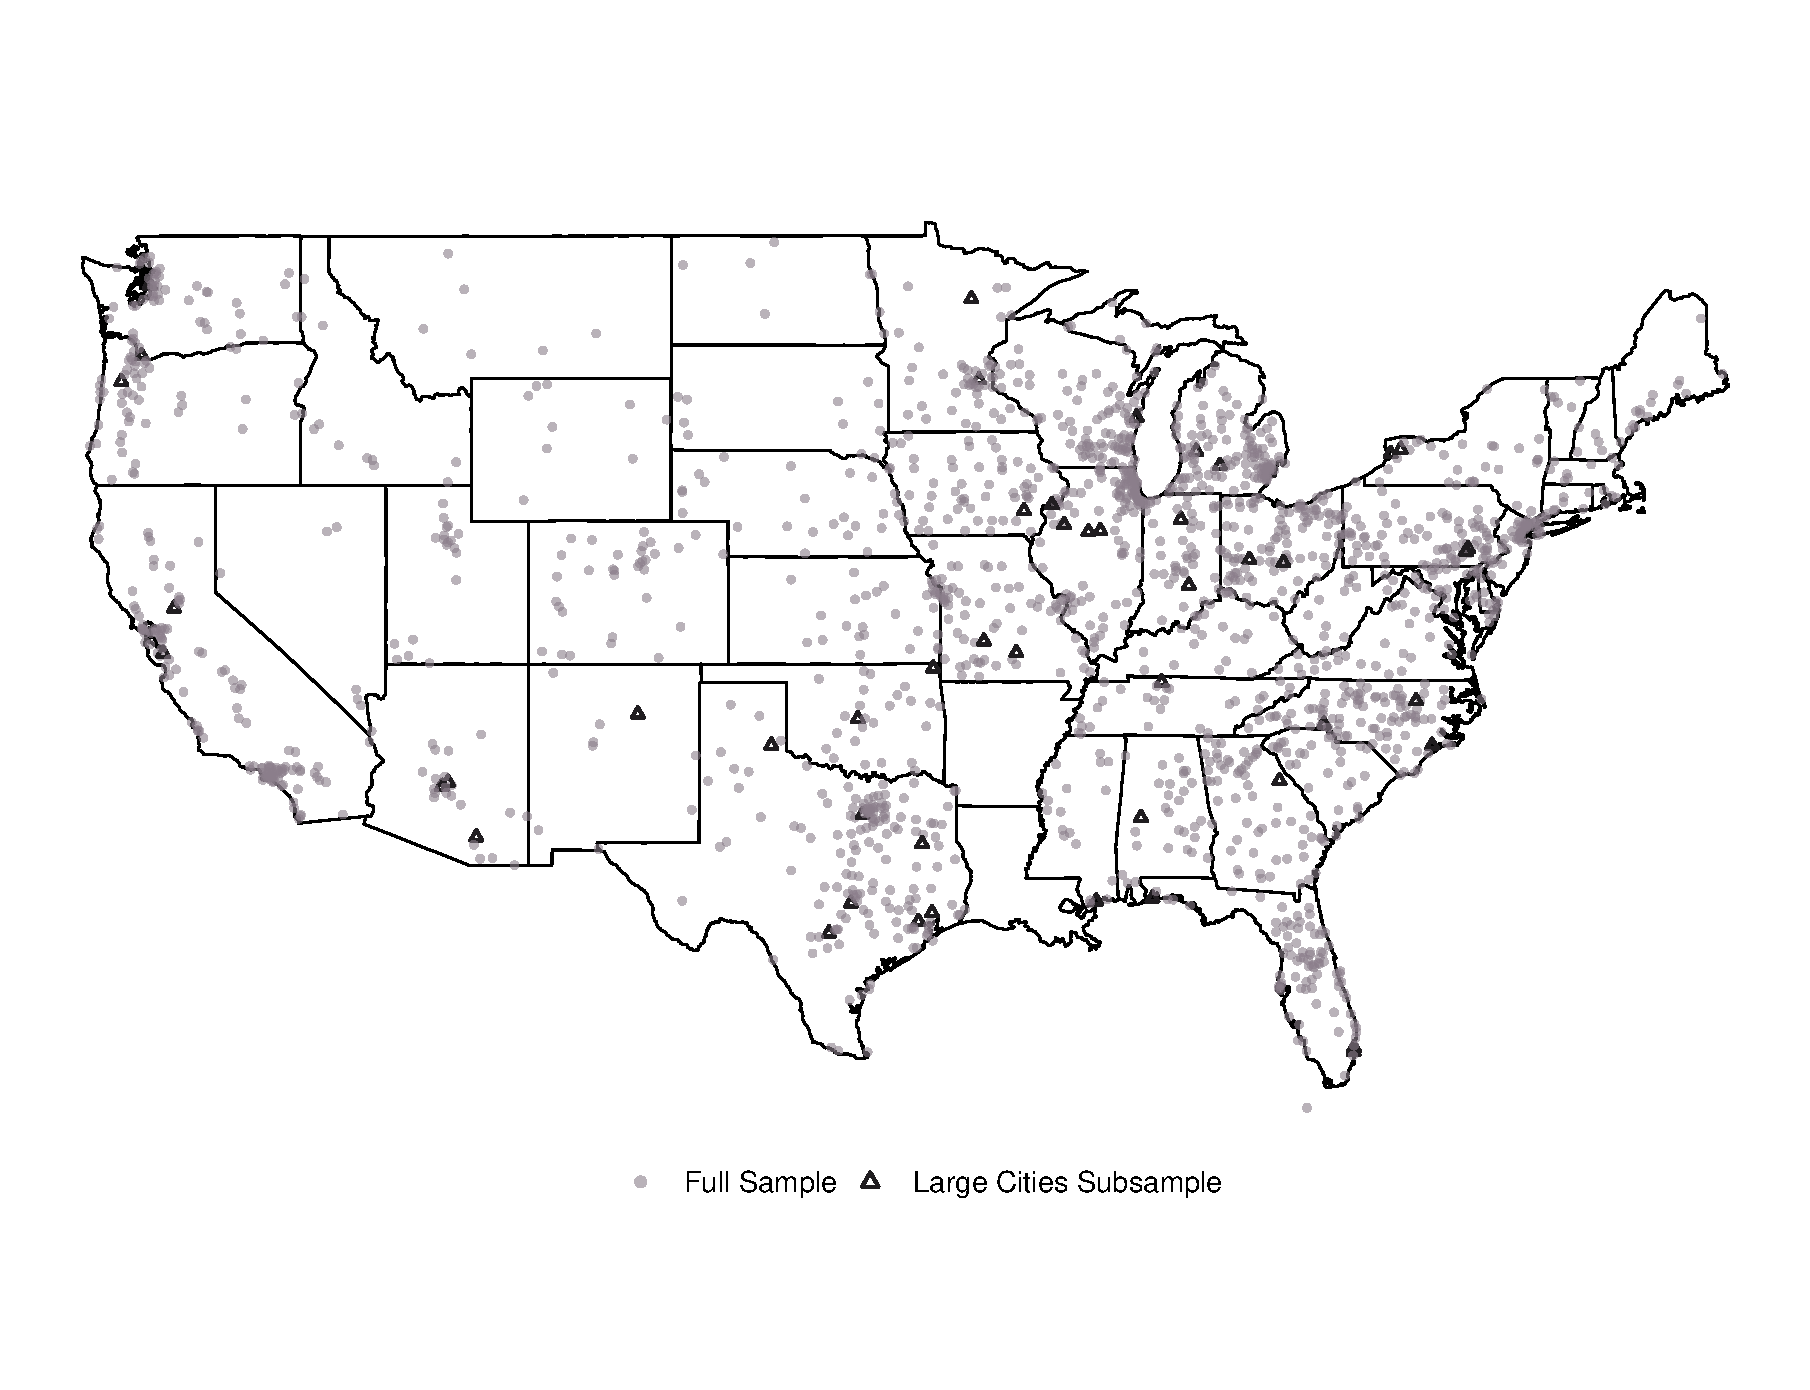
\includegraphics[width=\linewidth]{Figures/SampleMap.pdf}
    }
    \caption[Included Cities Map]{Cities included within my full sample (2,216) and large cities subsample (72).}
    \label{fig:SampleMap}
\end{figure}
 

As cities grow, the size and scope of both their internal governments and local services fundamentally change \citep{oliverDemocracySuburbia2001,oliverLocalElectionsPolitics2012}. Individuals within sparse rural areas such as Carlinville, IL (4,000) may interact inherently differently with local government and their services than individuals from a large urban center such as Chicago, IL (2.75 million) \citep{mooreMotivationsMobilizationComparing2022,debenedictis-kessnerStrategicGovernmentCommunication2022,lassenJurisdictionSizeLocal2011}. Moreover, from the large body of work examining the urban/rural divide within the U.S., an individual's partisan identity may also vary across these local contexts \citep{gimpelUrbanruralDivideResidential2023,nemereverContentiousFederalismSheriffs2021,scalaPoliticalPolarizationRuralUrban2017}. Thus, my results in the following sections may not map perfectly to these smaller American democracies. However, given that I identify clear trends within my larger sample and nearly 40\% of Americans still reside within similarly large cities, my proceeding analyses should provide valuable insight into mechanisms of local polarization and the relationship between local services and individuals' partisan identities.

\subsection{Reexamining Schools and Police}

For each of the 72 cities in my subset, I collected the reported 2018 violent and property crime rates reported by the city to the UCR program. While these measures help to alleviate concerns associated with county-level estimates, they still suffer from problems associated with using crime rates to gauge police performance. To supplement these rates, I also include the number of employees each city employs within its police department. I standardize these measures to the number of employees per 100,000 citizens to compare across municipalities of varying sizes. While the number of employees is not directly correlated to a city's ability to combat crime, it serves as a proxy for city-level spending on policing. For school performance, I use the identical standardized test scores used in the primary analysis.


 One of the critical problems present in my primary analysis above is that an individual's partisanship is not assigned randomly. One's partisan identity is closely correlated with various other identities influencing access to local services and selective residency. In an effort to combat concerns of endogenous confounding, I employ a procedure of covariate balanced propensity score weighting (CBPSW) as presented in \citet{imaiCovariateBalancingPropensity2014}. To improve matching, I match respondents on each of the previous controls included in the initial analysis in addition to city-specific objective performance measures. Using these weights, I then regress the effect of partisanship on evaluations of both local schools and police using both random state and municipality effects and present the results in \autoref{tab:CBPS}. Due to the variability associated with choosing weights, I opt to bootstrap the standard errors for my estimates. I recalculate the matches and fit the hierarchical model for each bootstrapped sample.


\begin{table}[H] \centering 
  \caption{Large City Analysis Using CBPS Weighting of Partisanship on Local Evaluations} 
  \label{tab:CBPS} 
  \scalebox{0.75}{
\begin{tabular}{@{\extracolsep{5pt}}lcc} 
\\[-1.8ex]\hline 
\hline \\[-1.8ex] 
 & \multicolumn{2}{c}{\textit{Service Evaluation:}} \\ 
\cline{2-3} 
\\[-1.8ex] & School & Police \\ 
\hline \\[-1.8ex] 
 Republican & $-$0.043 & 0.262$^{*}$ \\ 
  & (0.027) & (0.029) \\ 
  & & \\ 
 Constant & 0.240$^{*}$ & 0.345$^{*}$ \\ 
  & (0.063) & (0.042) \\ 
  & & \\ 
\hline \\[-1.8ex] 
Observations & 7,591 & 4,956 \\ 
AIC & 24,304.160 & 14,917.710 \\ 
\hline 
\hline \\[-1.8ex] 
\end{tabular} }
\begin{tablenotes}
    \item {\footnotesize Note: The above table presents the results of a CBPS Weighting with bootstrapped standard errors for my large cities sample. Bootstrapped standard errors are presented in parentheses. $^{*}$p$<$0.05}
\end{tablenotes}
\end{table} 

From the table above, the coefficients surrounding \textit{Republican} are again statistically significant at a $p<0.05$ level for police, while a similar pattern is not seen for schools. Additionally, the effect of partisanship in the case of police appears to be similar to my initial analysis despite the inclusion of additional city-specific measures. I should note, however,  that CBPSW does not completely solve all concerns of endogeneity as the process is still sensitive to large misspecifications of the modeling process. Accounting for all possible confounders associated with one's partisan identity and interaction with local services is nearly impossible for this form of observational study; however, this procedure provides more probable estimates than those generated by traditional forms of regression alone. 

\subsection{An Alternative to Schools}
There may be some concern that schools do not provide an adequate contrast to test my theory of polarization. Given trends following nationwide shutdowns in response to the COVID-19 pandemic, some may argue that schools are far more polarized than I posit earlier in this paper. Luckily, given my focus on larger cities, I can examine another prominent local service: roads. While roads may receive less media or political attention, they are a salient service most individuals interact with to some degree on a daily basis. One objective measure of roads is traffic congestion. Using historic traffic data provided by TomTom, a popular transportation and navigation service, I assigned each city an index measure for their average level of traffic for the year 2018. \textit{Traffic Index} is measured on a 0 to 100 scale and calculated--- through GPS data---by measuring the average additional travel time traffic congestion adds to a standard 30-minute trip within a given city. For ease of calculation and interpretability, I employ a hierarchical linear regression that includes state- and city-level random effects and display my results in the table below.

\begin{table}[H] \centering 
  \caption{Hierarchical Linear Regression of Local Roads  Evaluation on Partisan Identity: Full Results} 
  \label{} 
  \scalebox{0.75}{
\begin{tabular}{@{\extracolsep{5pt}}lc} 
\\[-1.8ex]\hline 
\hline \\[-1.8ex] 
 & \multicolumn{1}{c}{\textit{Service Evaluation:}} \\ 
\cline{2-2} 
\\[-1.8ex] & Roads \\ 
\hline \\[-1.8ex] 
  Republican & 0.030 \\ 
  & (0.026) \\ 
  & \\ 
 Traffic Index & $-$0.003 \\ 
  & (0.003) \\ 
  & \\ 
 Age & $-$0.005$^{*}$ \\ 
  & (0.001) \\ 
  & \\ 
 Gender (M) & 0.020 \\ 
  & (0.022) \\ 
  & \\ 
 Black & $-$0.175$^{*}$ \\ 
  & (0.033) \\ 
  & \\ 
 Income & 0.016$^{*}$ \\ 
  & (0.004) \\ 
  & \\ 
 Constant & $-$0.003 \\ 
  & (0.077) \\ 
  & \\ 
\hline \\[-1.8ex] 
Observations & 6,928 \\ 
State Random Effects & \ding{51} \\ 
Municipality Random Effects & \ding{51} \\
Additional Controls & \ding{51}\\
AIC & 18,191.980 \\ 
\hline 
\hline \\[-1.8ex] 
\end{tabular} }
\begin{tablenotes}
    \item {\footnotesize Note: The above table presents the results of a hierarchical linear regression with random effects. All respondents are nested within municipalities within states. Full regression results can be found within the appendix. Standard errors are presented in parentheses.$^{*}$p$<$0.05}
\end{tablenotes}
\end{table} 

The results from Table 3 above suggest that one's partisan identity does not appear to play a significant role in their evaluations of local roads. However, the average traffic conditions do not significantly affect an individual's evaluations either. This finding could be because individuals use alternative cues, such as pavement conditions, to measure road quality. Alternatively, individuals may not have a conception of the annual performance of roads and instead base their evaluations on road conditions immediately surrounding when the survey was fielded. If this were the case, annual measures of road conditions may be poor objective performance measures for local road quality. Despite this finding, the results surrounding partisanship support my theory of polarized local services. Additionally, these results align with previous work examining road conditions, such as \citet{arceneauxDoesFederalismWeaken2005} and \citet{debenedictis-kessnerHowAttributionInhibits2018}, which find an inconsistent correlation between road and traffic conditions and perceived mayoral performance.

\subsection{Party Position Taking or Elite Valence?}
While the results thus far have supported my claim that for polarized services, individuals' partisan identities bias their evaluations, it remains to be seen as the exact mechanism behind this bias. As mentioned previously in this paper, this bias could be individuals adopting their national party's stance towards a service (i.e., favorability in the case of policing); however, it could also be caused by some form of partisan penalty/reward depending on which party holds political control. To examine this possibility, I borrow from \citet{debenedictis-kessnerAccountabilityLocalEconomy2020} analysis of the effect of mayoral partisanship on municipal spending to record the partisanship of each city's mayor and governor as of 2018 for each city within my large city subsample. I opt to control for both state and local partisan control due to the potentially blurred lines of responsibility for some local goods. While work such as \citet{arceneauxFederalFaceVoting2006} suggests that individuals can make meaningful distinctions between levels of government, they also highlight that this ability depends on an individual's perceived responsibilities of local, state, and federal governments \citep{arceneauxDoesFederalismWeaken2005}. The growing trend of nationalization and politicization may lead individuals to view state and federal governments as increasingly responsible for some local policy areas. For the analysis,  I employ a similar hierarchical regression as before and present the results in \autoref{tab:MayorParty}. 

\begin{table}[H] \centering 
  \caption{Hierarchical Linear Regression of State and Local Co-partisanship on Local Service Evaluations} 
  \label{tab:MayorParty} 
  \scalebox{0.75}{
\begin{tabular}{@{\extracolsep{5pt}}lccc} 
\\[-1.8ex]\hline 
\hline \\[-1.8ex] 
 & \multicolumn{3}{c}{\textit{Service Evaluation:}} \\ 
\cline{2-4} 
\\[-1.8ex] & Police & Roads & Schools \\ 
\hline \\[-1.8ex] 
 Co-partisan Mayor & $-$0.038 & 0.013 & 0.042 \\ 
  & (0.034) & (0.032) & (0.030) \\ 
  & & & \\ 
 Co-partisan Governor & 0.015 & 0.045 & 0.052 \\ 
  & (0.031) & (0.025) & (0.028) \\ 
  & & & \\ 
 Republican & 0.246$^{*}$ & 0.023 & -0.065 \\ 
  & (0.038) & (0.033) & (0.033) \\ 
  & & & \\ 
 Constant & $-$0.057 & $-$0.021 & $-$0.630$^{*}$ \\ 
  & (0.122) & (0.081) & (0.085) \\ 
  & & & \\ 
\hline \\[-1.8ex] 
Observations & 4,750 & 6,846 & 6,908 \\ 
AIC & 12,635.960 & 18,002.590 & 18,953.690 \\ 
State Random Effects & \ding{51} & \ding{51} & \ding{51} \\ 
Municipality Random Effects & \ding{51} & \ding{51} & \ding{51} \\
Objective Measures & \ding{51} & \ding{51} & \ding{51} \\
Additional Controls & \ding{51} & \ding{51} & \ding{51} \\
\hline 
\hline \\[-1.8ex] 
\end{tabular}} 
\begin{tablenotes}
    \item {\footnotesize Note: The above table presents the results of a hierarchical regression for my large cities sample. Respondents are nested within cities and then states. Co-partisanship was determined by whether the respondent shared the party of the acting Governor or Mayor in 2018. Standard errors are presented in the parentheses. $^{*}$p$<$0.05}
\end{tablenotes}
\end{table} 

In the case of all three local services, co-partisanship with either the city's mayor or governor does not significantly affect one's evaluations of local services. Even in the case of police, an individual's evaluations appear to be based far more on their partisan identity rather than their shared partisanship with local officials. While these null results don't necessarily mean shared partisanship does not affect local evaluations, for polarized services, the party's average position matters far more. These null results may be partially explained by the lack of party competition often found within municipal governments \citep{bucchianeriPartyCompetitionCoalitional2020}.



\section{Conclusion}

At the beginning of this article, I argued that individuals' evaluations of municipal services are not necessarily based on the quality of the service or their access to it. Instead, some local services have become polarized, leading to partisan distortions of evaluations in the direction of party preferences. Through an analysis of local police and schools, I provided strong correlational evidence that the polarized discourse surrounding police has led Republicans to evaluate the service more positively than other outpartisans. Additionally, I showed how a similar process is absent in non-polarized cases of local schools and local roads. 

My work adds to our understanding of retrospective evaluations within local politics in several ways. First, it highlights how increased nationalization and partisan sorting may inhibit retrospective voting within a local context. Second, the data used in my analysis departs from the traditionally geographically narrow approaches used to examine local politics and expands my analysis to a national sample. Lastly, it adds to our broader understanding of how polarization shapes electoral accountability. As individuals become increasingly sorted along party lines, my work suggests that retrospective evaluations may become less and less likely at all levels of government.

These findings suggest that partisanship may play a far more prominent role in the realm of local politics than previously conceived. For policymakers, this conclusion is potentially problematic as individuals may begin holding local services accountable for national opinions rather than their objective performance. By doing so, individuals may incentivize policymakers to prioritize polarizing aspects of local services at the potential detriment of the service as a whole. This analysis of local evaluations raises several vital questions surrounding local accountability and responsiveness. Notably, for two of the three examined services, objective measures of the said service failed to impact an individual's evaluation significantly. Future work should examine how individuals construct these perceptions of local services and which measures impact which group's evaluations. Additionally, while I've shown that partisanship may shape local assessments, it remains unclear whether this translates into any policy or electoral change. Examining how local politics' nationalization and potential polarization affect municipal policy-making and spending should be an essential focus of future work.

